\section*{The dataset features}

\subsection*{RMM matrix}
Most of the features in the analysis are elements in the so called Rapidity-Mass (RMM) matrix inspired by the work of Chekanov \cite{Chekanov_2019}.
\par
!! Motivation for using such a matrix in machine learning $\to$ hint to highly uncorrolated feats!!
\par
Its composition is determined as a square matrix of $1 + \sum_{i=1}^{T}N_i$ columns and rows, where T is the total number of objects (i.e jets, electrons etc.),
and $N_i$ is the multiplicity of a given object. In the case of the same number of a given object for all objects, we can denote the RMM matrix as a 
TmNn matrix, where m is the multiplicity of T, and n is the number of particle per type. Thus there is already room for evaluation, as the combination of number of objects 
and the number of each object type highly affects the analysis as well as computational resources. Each cell in the matrix contains information about
either single og two particle properties. An example is shown in matrix \ref{eq:rmmmatrix}.

\begin{equation}\label{eq:rmmmatrix}
\begin{pmatrix}
    \boldsymbol{e}_{T}^{miss} & m_T(j_1) & m_T(j_2) &  m_T(e_1) &  m_T(e_2)\\
    h_L(j_1) & \boldsymbol{e_T}(j_1) & m(j_1, j_2) & m(j_1, e_1) & m(j_1, e_2)\\
    h_L(j_2) & h(j_2, j_1) & \delta \boldsymbol{e_T}(j_2)& m(j_2, e_1) & m(j_2, e_2)\\
    h_L(e_1) & h(e_1, j_1) & h(e_1, j_2) & \boldsymbol{e_T}(e_1) & m(e_1, e_2)\\
    h_L(e_2) & h(e_2, j_1) & h(e_2, j_2) & h(e_2, e_1) & \delta \boldsymbol{e_T}(j_2)\\
\end{pmatrix}
\end{equation}

In matrix \ref{eq:rmmmatrix} we have the RMM matrix for a T2N2 system, in other words we have two types of particles, jets and electrons, where each type has
two particles. The matrix itself is partitioned into three parts. The diagonal represents energy properties, the upper triangular represents mass properties, 
and the lower triangular represents longitudal properties related to rapidity. The diagonal has three different properties, $\boldsymbol{e_T^{miss}}$, $\boldsymbol{e_T}$ and $\delta\boldsymbol{e_T}$. 
$\boldsymbol{e_T^{miss}}$ is placed in the $(0,0)$ in the matrix. It accounts for the missing energy for the system, which is of high interest for this analysis due to
the search for heavy neutrinos. $\boldsymbol{e_T}$ is the transverse energy defined as 
\begin{equation*}
    \boldsymbol{e_T} = \sqrt{m^2 + p_T^2}
\end{equation*}
but for light particles such as electrons, this can be approximated to $\boldsymbol{e_T} \approx p_T$. $\delta\boldsymbol{e_T}$ is the transverse energy imbalance.
It is defined as 
\begin{equation*}
    \delta\boldsymbol{e_T} = \frac{E_T(i_n-1) - E_T(i_n)}{E_T(i_n-1) + E_T(i_n)}, \, n = 2, ..., N.
\end{equation*}
The first columm in the RMM matrix, with the exeption of the first element, is related to the longitudal property of the given particle. 
It is defined as
\begin{equation*}
    h_L(i_n) = C(\cosh{(y)} - 1),
\end{equation*}
where C is a constant to ensure that the average $h_L(i_n)$ values do not deviate too much from the ranges of the invariant masses of the transverse masses, found to be $0.15$\cite{Chekanov_2019}. 
y is the rapidity of the particle, and $i_n$ is the particle number. On the lower triangle we have the longitudal properties of the combinations of particles. Similar to $h_L(i_n)$,
this property is defined as 
\begin{equation*}
    h(i_n, j_k) = C(\cosh{(\Delta y)} - 1),
\end{equation*}
where $\Delta y = y_{i_n} - y_{j_k}$ is the rapidity difference for particle $i_n$ and $j_k$.


\subsection*{MonteCarlo and data comparison}\label{sec:mcdatacomp}

Before we can start the analysis, we need to compare the MonteCarlo and data. This is done by comparing the distributions of the features in the MonteCarlo and data.

\begin{figure}
    \centering
    \begin{subfigure}{.6\textwidth}
        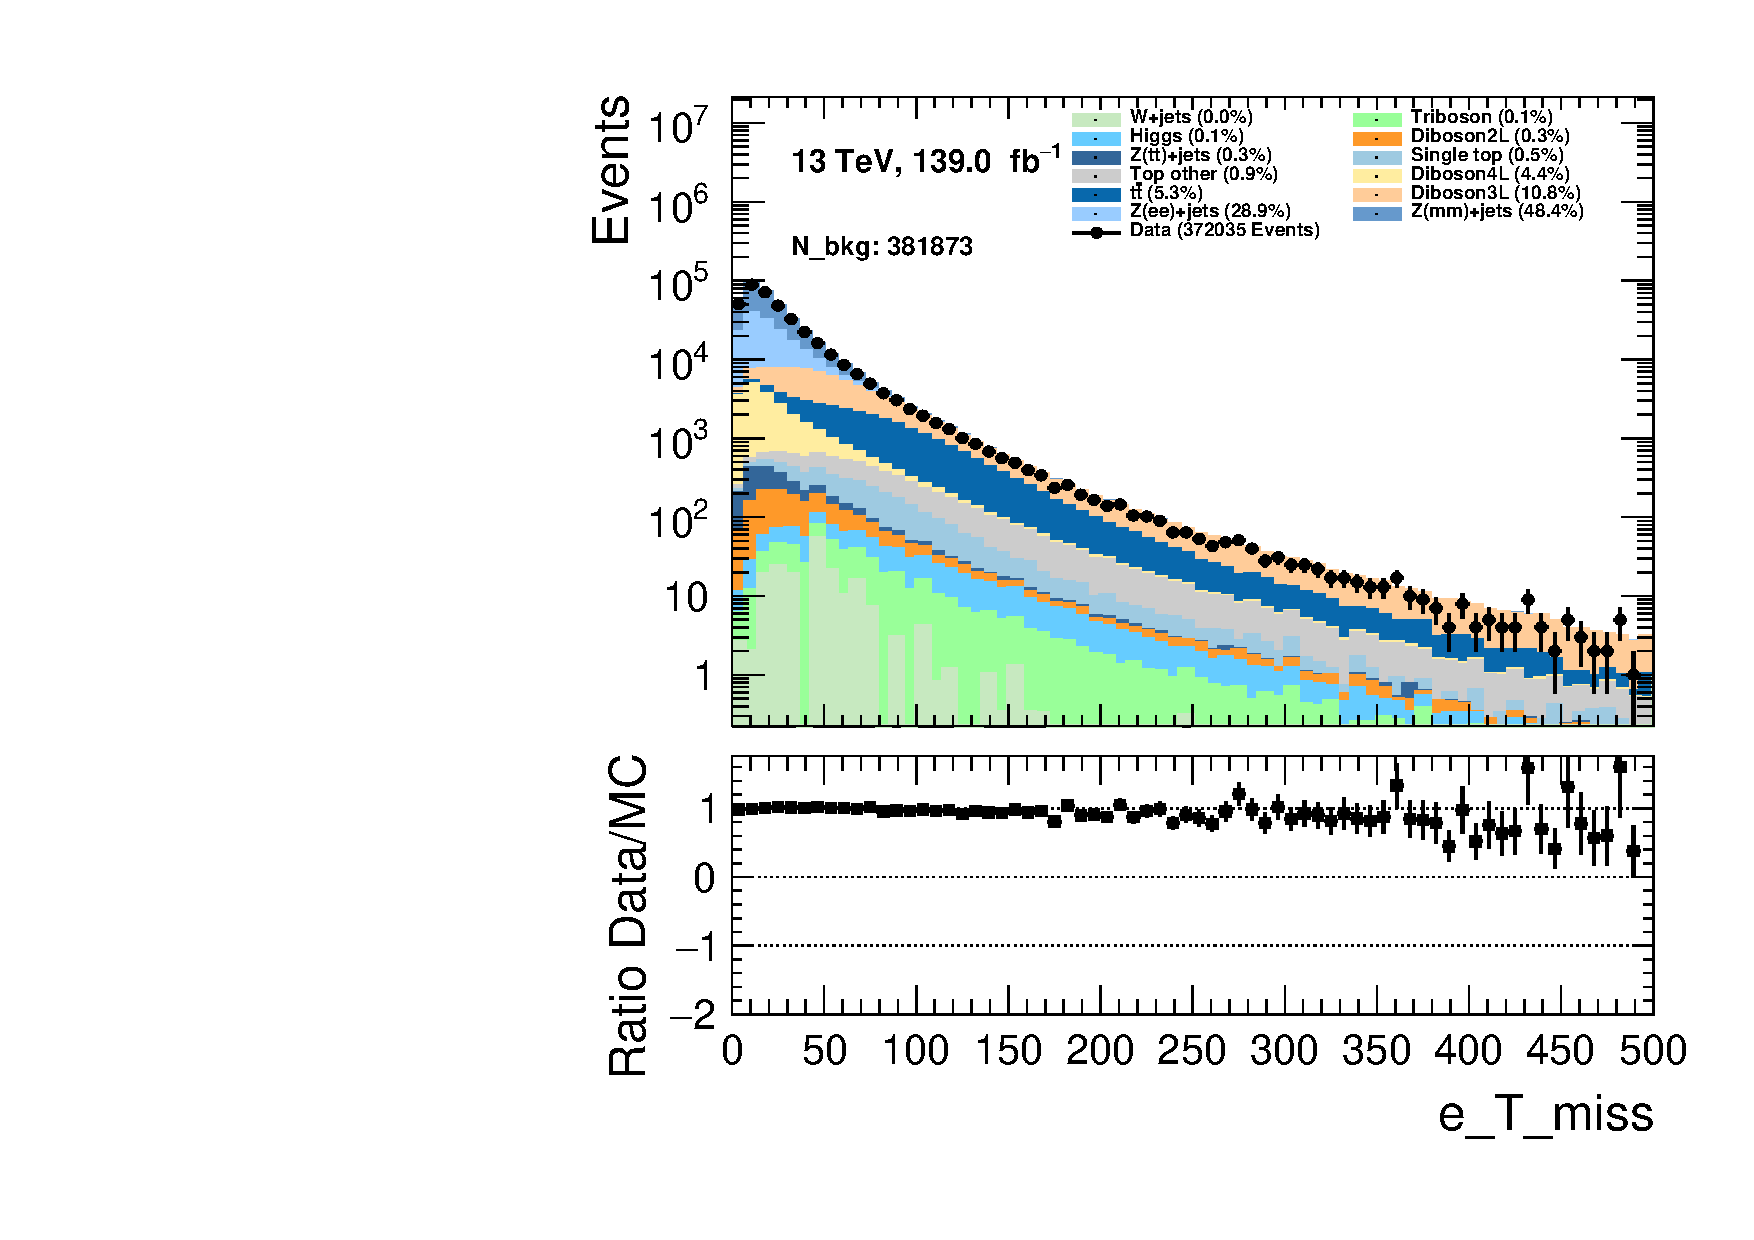
\includegraphics[width=\textwidth]{Figures/MC_Data_comp/e_T_miss.pdf}
        \caption{Missing transverse energy for the three lepton final state. The histogram contains the entire Run 2 dataset.}
        \label{fig:etmiss}
    \end{subfigure}
    \hfill
    \begin{subfigure}{.6\textwidth}
        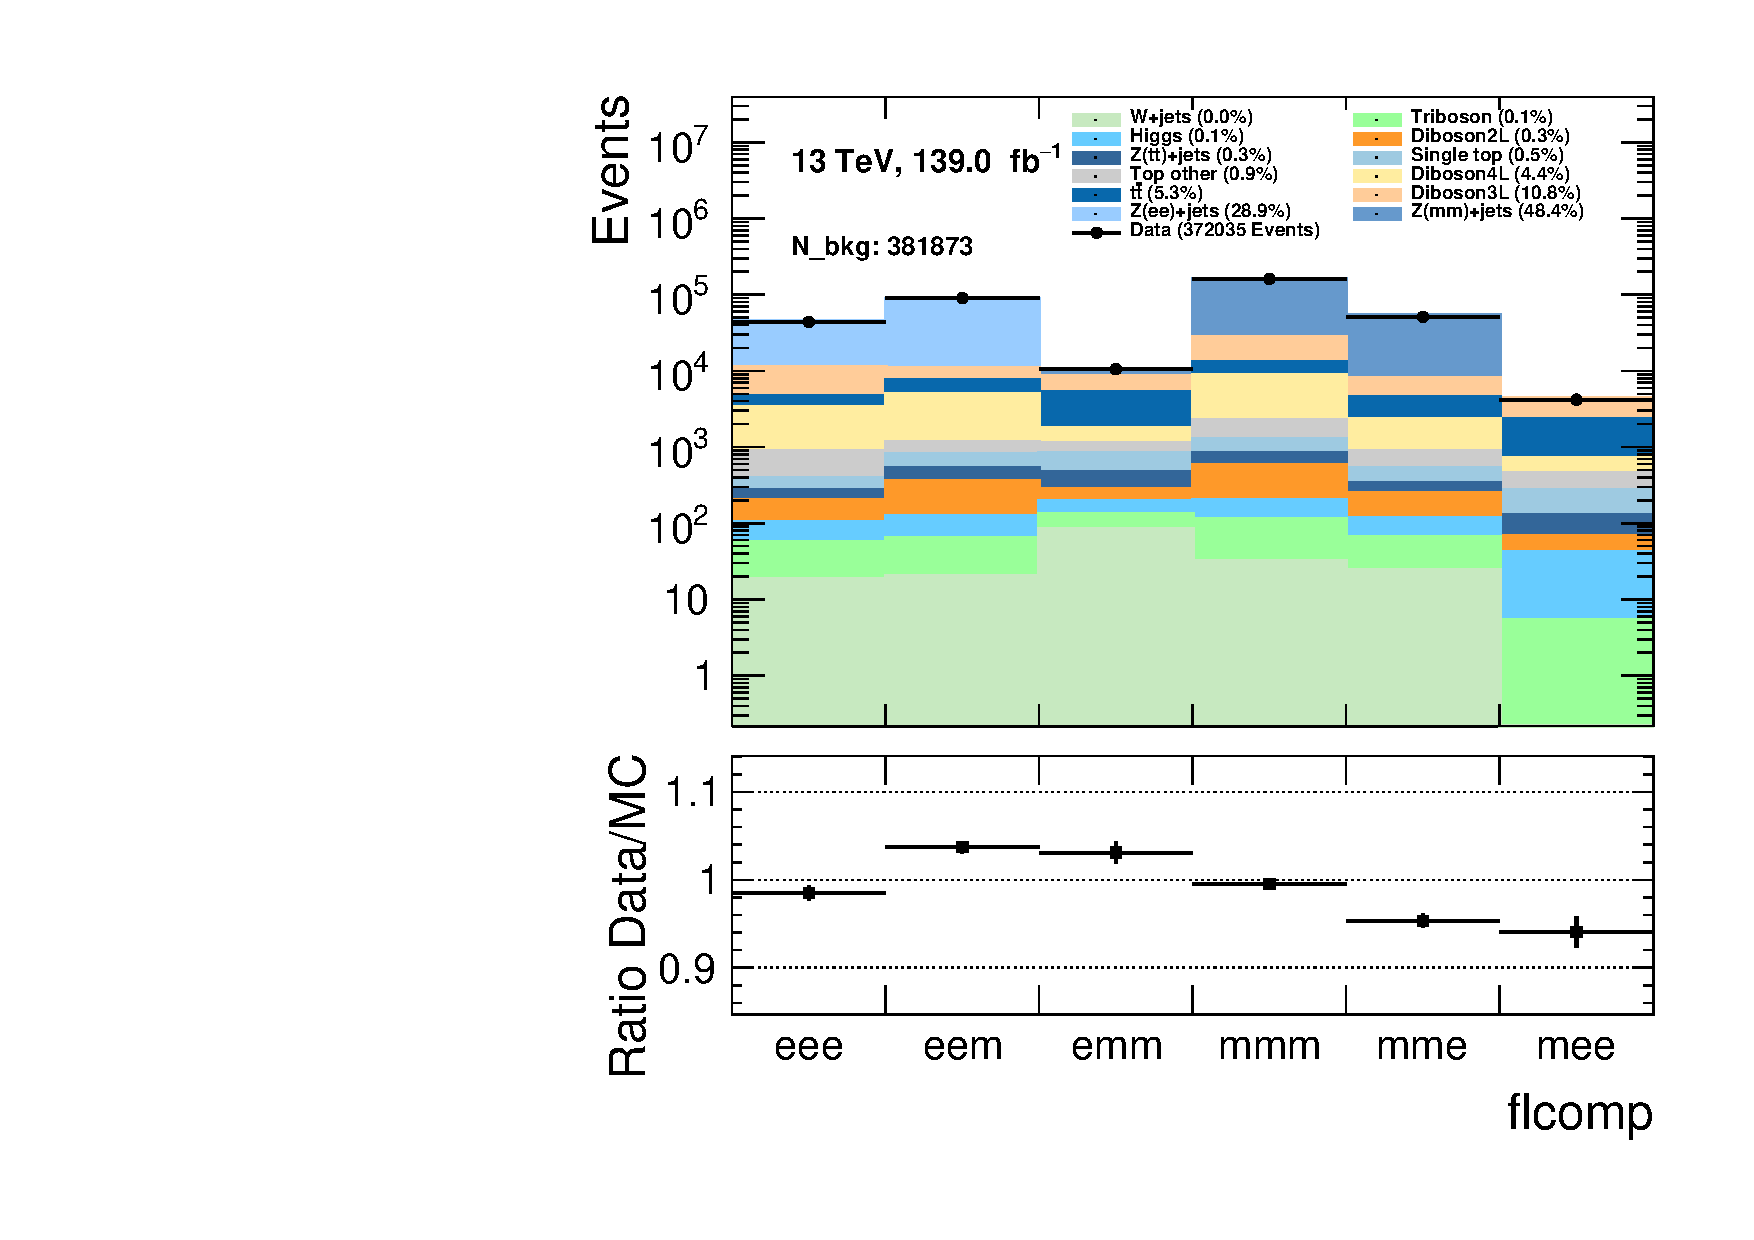
\includegraphics[width=\textwidth]{Figures/MC_Data_comp/flcomp.pdf}
        \caption{Flavor combination for the three lepton final state. This histogram only contains the flavor combinations for the good leptons, denoted $lep_{SG}$. The histogram contains the entire Run 2 dataset. }
        \label{fig:flcomp}
    \end{subfigure}
    \hfill        
    \caption{Comparison of the MonteCarlo and data for the three lepton final state with the features $e_{T}^{miss}$ and flavor composition.
    }
    \label{fig:MC_Data_comp}
\end{figure}

In figure \ref{fig:MC_Data_comp} two features have been selected to vizualize the comparison between Monte Carlo and ATLAS data, $e_T^{miss}$ and $flcomp$. 
We see that both $e_T^{miss}$ and $flcomp$ satisfy a good ratio between Monte Carlo and ATLAS data, thus we can safely move forward with the analysis. 
All features were checked, and can be found in appendix B.